

%!TEX root = ../Notes.tex
\section{Continuity, metric spaces, and open balls} We'd like to be able to talk about continuity in metric spaces (not just the reals).
\begin{definition}
	Let $(M_1, d_1)$ and $(M_2, d_2)$ be metric spaces and $a \in M_1$. Let $f:M_1 \rightarrow M_2$. We say $f$ is {\bf continuous} at a if $\forall \epsilon > 0$ there exists a $\delta > 0$ such that $\forall x\in M_1$ with $d_1 (x,a) <\delta$ then $d_2 (f(x), f(a))<\epsilon$. 
\end{definition}

%\begin{figure}[ht!]
\[ 
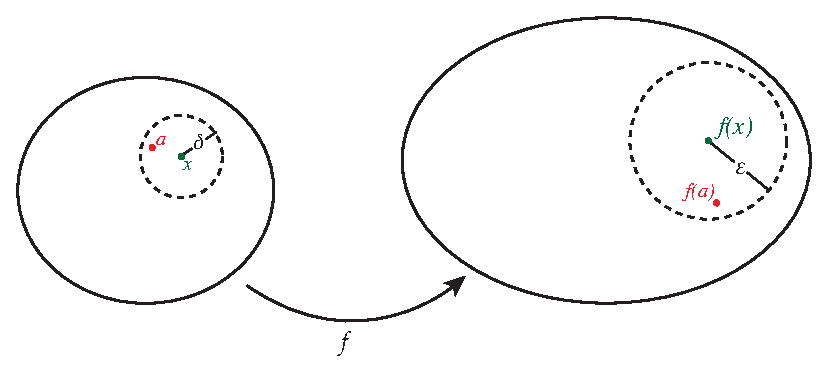
\includegraphics[width=300pt]{images/continuity_etc/continuous_metric_space}\]

%    \caption{For any $a$ such that $d_1(x,a) < \delta$, we have $d_2(f(x), f(a)) < \epsilon$.}
%\end{figure}
\begin{definition}
	Let (M,d) be a metric space and $a\in M$. The {\bf open ball of radius $\epsilon >0$ about $a$} is defined to be
	\[B_\epsilon (a) = \{x\in M\ |\ d(x,a)<\epsilon \}\]
\end{definition}

We can redefine `continuous' in terms of open balls: 
\begin{definition}
	A function $f:X\to Y$ is {\bf continuous} at $a\in X$ iff $\forall\epsilon > 0$ there exists a $\delta >0$ such that if $x\in B_\delta (a)$ then $f(x) \in B_\epsilon (f(a))$.
	
	In other words, $f$ is continuous at $a$ iff for every $\epsilon > 0$ there is some $\delta > 0$ such that $f(B_\delta (a)) \subseteq B_\epsilon (f(a))$. 
\end{definition}

%\begin{figure}[ht!]
\[ 
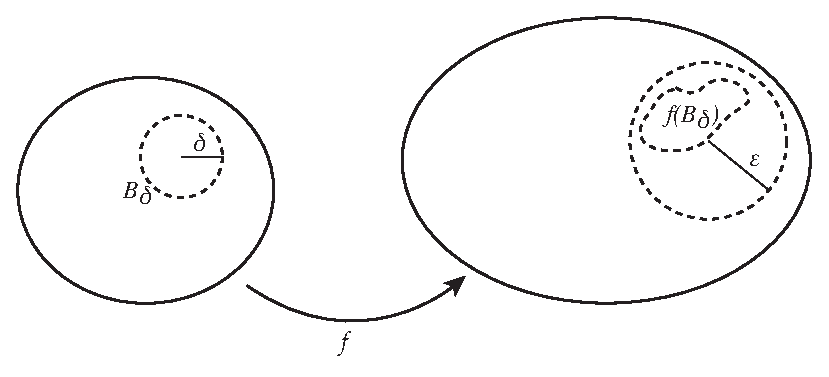
\includegraphics[width=300pt]{images/continuity_etc/continuous_metric_space_balls}\]

%    \caption{For any $\epsilon$, there is some $\delta$ such that $f(B_\epsilon(x))\subseteq B_\delta$.}
%\end{figure}
It should be noted that open balls don't always look like open balls...
\begin{example}
	$M =$ upper half of plane with usual distance
	
	%\begin{figure}[ht!]
	\[ 
	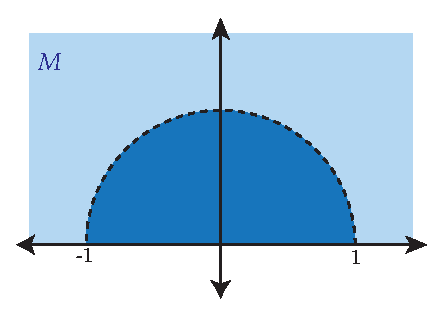
\includegraphics[width=240pt]{images/continuity_etc/upper_half_plane_ex}\]
	
	%    \caption{This half-circle is the intersection of an open set with $M$, so it is open.}
	%\end{figure}
	Because the dark-blue semicircle is the intersection of the open set $\{(x,y)\in\R^2\ |\ x^2+y^2<1\}$ with $M$, it is open in $M$. 
\end{example}
\begin{example}
	In $\R$ with the discrete metric, $B_1 (47) = {47}$ and $B_2 (47) = \R$. 
\end{example}
\begin{example}
	[Comb metric] Under the comb metric, $B_{\frac{1}{2}} ((0,1))$ is just an interval along the y-axis starting at $(0,1)$.
	
	$B_2 ((0,1)$ is everything on the comb below the line of slope $-1$ that connects points $(0,1)$ and $(1,0)$. Since it's an open ball, the line is not contained in the ball.
	\[ 
	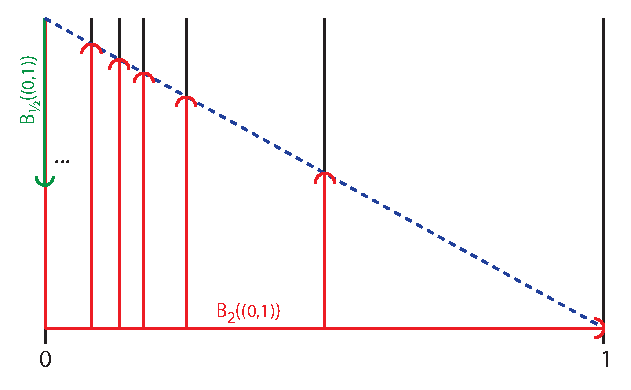
\includegraphics[width=360pt]{images/continuity_etc/comb_metric_balls} \]
\end{example}

Note: Balls are not closed under $\bigcup$ and $\bigcap$ - in $\R^2$, $B_{1}((0,0)) \cap B_{1/2}((1,0))$ and $B_{1}((0,0))\cup B_{1/2}((1,0))$ are not balls.

\section{Open sets} 
\begin{definition}
	Let $(M,d)$ be a metric space. A set $U \subseteq M$ is said to be {\bf open} if $\forall a\in U$ there exists an $\epsilon >0$ such that $B_\epsilon (a) \subseteq U$. 
\end{definition}
\begin{example}
	Every subset of a set $M$ under the discrete metric is open.
\end{example}

\mbox{ }
\begin{smallfact}
	In a metric space, open balls are open sets. 
\end{smallfact}
\proof{ Let $a \in M$ and $\epsilon >0$. We want to show that $B_\epsilon (a)$ is open. That is, we want to show that $\forall x \in B_\epsilon (a)$ there exists an $r>0$ such that $B_r (x) \subseteq B_\epsilon (a)$.

Let $x \in B_\epsilon (a)$ and let $r < \epsilon - d(x,a)$ and $r > 0$. We claim that $B_r (x) \subseteq B_\epsilon (a)$. 

Let $y \in B_r (x)$. Then $d(y,a)\leq d(y,x) + d(x,a) < \epsilon - d(x,a) + d(x,a)= \epsilon$.

Therefore, $B_r (x) \subseteq B_\epsilon (a)$ }
\begin{definition}
	Let
	\[\bigcup_{i \in I} U_i = \{x \in U_i\ |\ i \in I\}\]
\end{definition}
\pagebreak
\begin{theorem}
	(the ``open sets are nice" theorem)
	
	Let $F$ be the family of open sets in a metric space $(M,d)$. Then: 
	\begin{enumerate}
		\item $M$, $\emptyset \in$ $F$ 
		\item If U, V $\in$ F then U $\cap$ V $\in$ F 
		\item If $\forall i \in I$, $U_i \in F$ then $\bigcup_{i \in I} U_i \in F$ 
	\end{enumerate}
\end{theorem}
\begin{proof}
	\begin{enumerate}
		\item Let $x\in M$, and $\epsilon = 47$. By definition,
		\[B_{47} (x) = \{y\in M\ |\ d(x,y)<47\} \subseteq M\]
		Also, trivially $\forall x\in \emptyset$ there exists an $\epsilon > 0$ such that $B_\epsilon (x) \subseteq \emptyset$. Therefore, $M$ and $\emptyset$ are open, and so $M, \emptyset\in F$.
		
		\item Let $x\in U\cup V$, let $r_1 >0$ such that $B_{r_1} (x) \subseteq U$, and let $r_2 >0$ such that $B_{r_2} (x) \subseteq V$. Let $r = \min\{r_1, r_2 \}$. Then clearly $B_r (x) \subseteq B_{r_1} (x) \subseteq U$ and $B_r (x) \subseteq B_{r_2} (x) \subseteq V$. Thus $B_r (x) \subseteq U \cap V$ as desired.
		
		\item Let $x \in \bigcup_{i\in I} U_i$. We want to show that there exists an $r>0$ such that $B_r (x) \subseteq \bigcup_{i\in I} U_i$. 
		
		Because $x\in \bigcup_{i\in I} U_i$, there exists an $i_0 \in I$ such that $x\in U_{i_0}$. Then there must exist an $r>0$ such that $B_r (x) \subseteq U_{i_0}$. Then
		\[B_r (x) \subseteq U_{i_0} \subseteq \bigcup_{i\in I} U_i\]
		and hence $\bigcup_{i\in I} U_i\in F$. 
	\end{enumerate}
\end{proof}
\begin{definition}
	If $f:X \to Y$ and $U \subseteq Y$ then $f^{-1} (U) = \{x\in X\ |\ f(x) \in U\}$. 
\end{definition}
\begin{theorem}
	Let $(M_1, d_1)$ and $(M_2, d_2)$ be metric spaces and $f: M_1 \to M_2$. Then $f$ is continuous if and only if for every $U \subseteq M_2$ that is open in $(M_2, d_2)$, $f^{-1} (U)$ is open in $(M_1, d_1)$. 
\end{theorem}
\begin{proof}
	\begin{itemize}
		\item[$(\Rightarrow)$] Suppose $f$ is continuous. Let $U \subseteq M_2$ be open. We want to show that $\forall x \in f^{-1} (U)$ there exists an $r>0$ such that $B_r (x) \subseteq f^{-1} (U)$.
		
		Let $x\in f^{-1} (U)$. Since $f(x)\in U$ and $U$ is open, there exists $\epsilon >0$ such that $B_\epsilon (f(x)) \subseteq U$. Since $f$ is continuous there exists an $r>0$ such that
		\[f(B_r (x)) \subseteq B_\epsilon (f(x)) \subseteq U\]
		
		Thus, $f^{-1} (f(B_r (x))) \subseteq f^{-1} (U)$. Therefore $B_r (x) \subseteq f^{-1} (f(B_r (x))) \subseteq f^{-1} (U)$ as desired.
		
		\item[$(\Leftarrow)$] Suppose that for all open $U\subseteq M_{2}$, $f^{-1}(U)$ is open in $M_{1}$. Let $p \in M_{1}$. We want to show that $f$ is continuous at $p$.
		
		Let $\epsilon > 0$. $B_{\epsilon}(f(p))$ is open, so $f^{-1}(B_{\epsilon}(f(p)))$ is open. $p\in f^{-1}(B_{\epsilon}(f(p)))$, so $\exists$ $\delta>0$ such that $B_{\delta}(p)\subseteq f^{-1}(B_{\epsilon}(f(p)))$.
		
		$f(B_{\delta}(p))\subseteq f(f^{-1}(B_{\epsilon}(f(p))))=B_{\epsilon}(f(p))$, so $f$ is continuous at $p$, and thus everywhere. $\blacksquare$ 
	\end{itemize}
\end{proof}

We've proven a small fact: 
\begin{smallfact}
	If $f : M_{1} \rightarrow M_{2}$, then $f$ is continuous if for all $p\in M_{1}$, and for all $\epsilon>0$ $f^{-1}(B_{\epsilon}(f(p)))$ is open. 
\end{smallfact}
